\documentclass[12pt]{report}

\usepackage{titlesec}
\usepackage{graphicx}
\usepackage{multibib}
\usepackage{amsthm}
\usepackage{tikz}
\usepackage{algorithm2e}
\usepackage[a4paper, total={6in, 9in}]{geometry}
\titleformat{\chapter}[display] {\normalfont\Huge\bfseries}{\chaptertitlename\ \thechapter}{0pt}{\Huge}
\titlespacing{\chapter}{0cm}{0cm}{1cm}
\theoremstyle{definition}
\newtheorem*{example}{Example}
\theoremstyle{definition}
\newtheorem*{algo}{Algorithm}
\theoremstyle{definition}
\newtheorem*{method}{Method}
\RestyleAlgo{ruled}
\counterwithout{figure}{chapter}



\begin{document}


\begin{titlepage}
    \newcommand{\HRule}{\rule{\linewidth}{0.5mm}} %Horizontal line break%
    \center
    \textsc{\LARGE Université Toulouse III Paul Sabatier}\\[2.5cm]
    \textsc{\Large Master Thesis Report}\\[0.5cm]
    \textsc{\large Computer Science for Aerospace}\\[2.5cm]

    \HRule\\[0.5cm]
    {\huge \bf Multivariate Decision Tree Classification}\\[0.5cm]
    \HRule\\[1.5cm]

    \begin{minipage}{0.4\textwidth}
		\begin{flushleft}
			\large
			\textit{Author}\\
			Dany Morales
		\end{flushleft}
	\end{minipage}
    \begin{minipage}{0.4\textwidth}
		\begin{flushright}
			\large
			\textit{Supervisors}\\
			Martin Cooper\\
            Emmanuel Hebrard
		\end{flushright}
	\end{minipage}

    \vfill
    \large January 2024

    \includegraphics[width=0.5\textwidth]{logo.png}
\end{titlepage}

\newpage
\tableofcontents

\newpage
\chapter*{Introduction}
\paragraph{} This report is about the work achieved during the M2 Computer Science for Aerospace thesis.
The supervisors are Mr. Martin Cooper at the \textit{Institut de Recherche en Informatique de Toulouse (IRIT)}
and Mr. Emmanuel Hebrard at the \textit{Laboratoire d'Analyse et d'Architecture des Systèmes in Toulouse (LAAS)}.
The goal of this master thesis is to implement a way for the decision tree classification algorithm called
Blossom to support multivariate decision trees. In this report, we will first introduce useful notions
related to this topic with a brief state of the art of decision tree classification. Afterwards, we will
present what we have done so far and the results we have obtained. Finally we will overview what we are
planning for the rest of the thesis.
%a bit more infos ---> continuation of internship, more context for the actual work, talk about work of
%Mr Cooper and Mr. Hebrard


\chapter{Preliminary research}
\section{Decision trees}

\paragraph{} A decision tree is a type of tree that helps to make a choice given a certain problem. In figure
\ref{fig:tree}, the problem would be if it is possible to go play outside depending on the weather.

\begin{figure}[h]
    \centering
    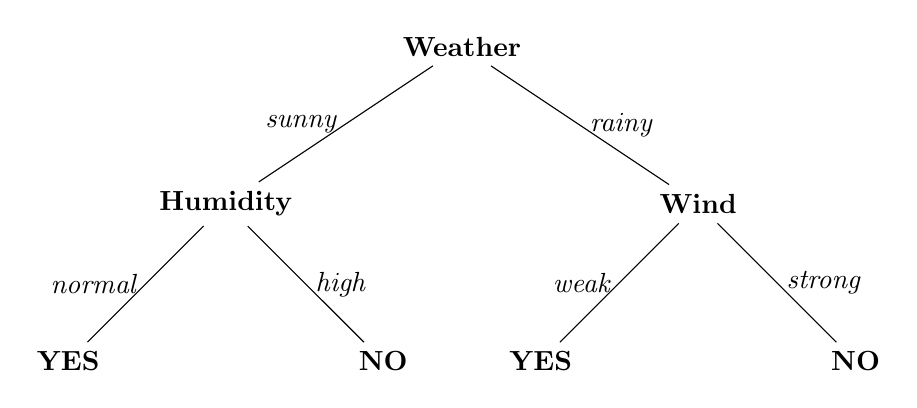
\begin{tikzpicture}
        [
            level 1/.style = {level distance = 2cm, sibling distance = 6cm},
            level 2/.style = {sibling distance = 4cm}
        ]
        
        \node {\bf Weather}
            child {node {\bf Humidity}
            child {node {\bf YES}
            edge from parent node [left] {\it normal}}
            child {node {\bf NO}
            edge from parent node [right] {\it high}}
            edge from parent node [left] {\it sunny}} 
            child {node {\bf Wind}
            child {node {\bf YES}
            edge from parent node [left] {\it weak}}
            child {node {\bf NO}
            edge from parent node [right] {\it strong}}
            edge from parent node [right] {\it rainy}};
    \end{tikzpicture}
    \caption{``\textit{Play outside}'' decision tree}
    \label{fig:tree}
\end{figure}

\paragraph{} This decision tree is the result of the classification of the dataset in figure
\ref{fig:dataweather}.

\begin{figure}[h]
    \centering
    \begin{tabular}{||c c c c||} 
    \hline
    Weather & Humidity & Wind & Play\\[0.5ex]
    \hline\hline
    Sunny & High & Strong & NO\\ 
    Sunny & Normal & Strong & YES\\
    Rainy & High & Strong & NO\\
    Rainy & High & Weak & YES\\ 
    \hline
    \end{tabular}
    \caption{``\textit{Play outside}'' dataset}
    \label{fig:dataweather}
\end{figure}

\paragraph{} According to this decision tree, if it is sunny and the humidity is normal, we can play outside.
On the other hand, if there is rain and wind, we cannot play outside. Weather, humidity and wind are called
features. This tree has two outcomes also called classes: YES and NO. On each node or decision node, the dataset
is split into two subsets depending on a chosen feature. At the root, we split on the weather feature: each
value of the dataset with $weather = sunny$ will be on the left subtree and each value of the dataset with
$weather = rainy$ will be on the right subtree.

\section{Classification concepts} %remove maybe?%
\paragraph{} A decision tree can be built from a dataset, the root node represents the entire set, then it is
divided into two more homogeneous sets creating two new decision nodes. We repeat this process recursively
until a specified maximum depth or until the subset is considered \textbf{pure}.
\paragraph{} The purify of a set can be defined with several metrics. A naïve way of defining it would be for
example, in a set in which there is a gender feature composed of 70\% males and 30\% females, the purity of
the set would be 70\%. We will introduce two methods used to find the purity of a set used in various algorithms.
\begin{method}[Information gain]
    The information gain uses the entropy in order to establish the purity of two subsets. If the information
    gain is high, the two subsets are considered pure, on the contrary, low information gain means impure
    subsets.
    \begin{displaymath}
        InformationGain(S) = H(S) - [H(S_1) + H(S_2)]
    \end{displaymath}
    \paragraph{} $S_1$ and $S_2$ are the two subsets resulting from spliting $S$. The entropy $H$ of a set $S$
    with $J$ classes can be defined using the Shannon entropy where $p_i$ is the probability of the class $i$
    to happen.
    \begin{displaymath}
        H(S) = - \sum_{i=1}^{J} p_i log_2 p_i
    \end{displaymath}

\paragraph{} This means that a set with a large entropy is not pure meanwhile a small entropy signifies a
better purity. A set with an entropy of zero is pure i.e. only one class is remaining which also means this
is a leaf in the decision tree. If a split is good, $S_1$ and $S_2$ will have a small entropy compared to the
parent set $S$ thus the information gain will be high.
\end{method}

\begin{method}[Gini impurity]
    An another way of computing the purity of set is using the Gini index. It measures the probability for a
    random element of the set to be misclassified.
    \begin{displaymath}
        G(S) = 1 - \sum_{i=1}^{J} p_i^2
    \end{displaymath}
\paragraph{} A value of zero means that all instances of a set have the same class i.e. the set is pure.
When spliting a set, we must do a weighted average of the Gini index for every subset. If this average is lower
than the Gini index of the parent set, this means the split is good.
\end{method}

\paragraph{} Both these methods are viable and provide different results depending on the implementation but
the choice of impurity measurement can have a significant impact. Other indicators exist such as variance 
reduction or chi-square however, the algorithms we will consider mainly use information gain and gini index.

\section{Multivariate decision trees}
\paragraph{} ``A multivariate decision tree is a decision tree in which the condition tested at a node is a constraint on
any number of features \cite{multivariate-explaining}.'' The principles of information gain, entropy and Gini
impurity are still valid but, as we introduce another condition to test, finding the best split for each
decision node becomes more costly to compute.

\begin{figure}[h]
    \centering
    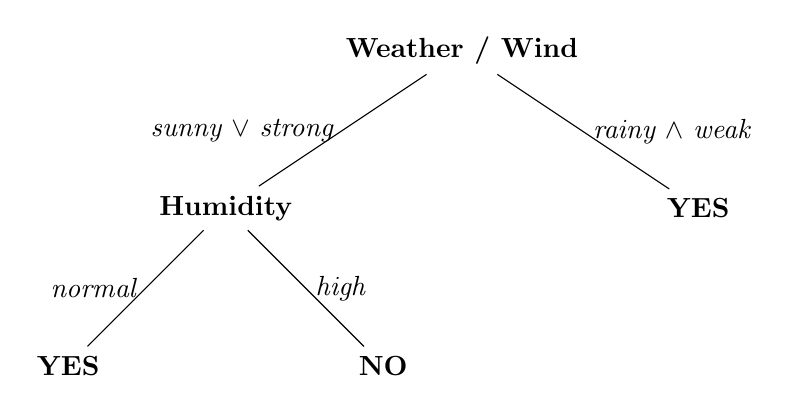
\begin{tikzpicture}
        [
            level 1/.style = {level distance = 2cm, sibling distance = 6cm},
            level 2/.style = {sibling distance = 4cm}
        ]
        
        \node {\bf Weather / Wind}
            child {node {\bf Humidity}
            child {node {\bf YES}
            edge from parent node [left] {\it normal}}
            child {node {\bf NO}
            edge from parent node [right] {\it high}}
            edge from parent node [left] {\it sunny $\lor$ strong}} 
            child {node {\bf YES}
            edge from parent node [right] {\it rainy $\land$ weak}};
    \end{tikzpicture}
    \caption{``\textit{Play outside}'' multivariate decision tree}
    \label{fig:multitree}
\end{figure}

\paragraph{} This is a possible multivariate decision tree that classifies the dataset in figure \ref{fig:dataweather}.
The root node test condition is on both the weather and wind features. The left child contains the subset
satisfying the condition $(weather=sunny \lor wind=strong)$ and the right child contains the subset satisfying
the negation i.e. $(weather=rainy \land wind=weak)$. It is important to note that the number of features a
condition is testing do not have to be the same at every node.


\chapter{State of the art}
\section{Decision tree learning} %use this part for explaining classification and talk about complexity here%
\section{Heuristic algorithms} %update to add which purity measure each algo uses%
\begin{algo}[ID3]
    Iterative Dichotomiser (1986) is a greedy algorithm developed by Ross Quilan that splits the dataset
    using the information gain metric. This algorithm is the one we implemented in Python during our TER.\\
    $\mathcal{D}$ is the input dataset and $\mathcal{F}$ contains the features of a given set.

\begin{algorithm}
    \caption{ID3}\label{alg:two}
    \DontPrintSemicolon
    \KwData{$\mathcal{D}$}
    \SetKwFunction{BuildTree}{BuildTree}
    \SetKwFunction{BestSplit}{BestSplit}

    \SetKwProg{Bn}{Function}{:}{}
    \Bn{\BuildTree{$S, depth_{max}$}}{
        \If{$depth \leq depth_{max}$}{
            $(left, right) \gets \BestSplit{S}$\;
            $subtree_L \gets \BuildTree{left}$\;
            $subtree_R \gets \BuildTree{right}$\;
            \KwRet $Node(subtree_L, subtree_R)$
        }
        \KwRet $Leaf(S)$\;
    }
    \;
    \SetKwProg{Sn}{Function}{:}{}
    \Sn{\BestSplit{$S$}}{
        $IG \gets 0$

        \ForEach{$f \in \mathcal{F}$}{
            $\mathcal{T} \gets thresholds()$

            \ForEach{$t \in \mathcal{T}$}{
                $(l, r) \gets split(S, t, f)$

                \If{$IG \neq \max(IG, infogain(S, l, r))$}{
                    $(left, right) \gets (l, r)$\;
                    $IG \gets infogain(S, l, r)$
                }
            }
        }
        \KwRet $(left, right)$
    }
    \;

    \BuildTree{$\mathcal{D}$}
\end{algorithm}

\begin{itemize}
    \item $thresholds()$ gives all the possible values of a feature $f$
    \item $split(S, t, f)$ splits the dataset $S$ at the treshold value $t$ on the feature $f$
    \item $infogain(S, l, r)$ computes the information gain of the split, so the set $S=l+r$ 
\end{itemize}
\end{algo}

\begin{algo}[C4.5]
    Developed in 1993 by Ross Quilan, it is the successor of ID3 and works the same way. It is an extension
    of ID3 offering several improvements. This version can handle both continuous and discrete values.
    Some post processing is added called pruning: it eliminates branches that do not provide additional
    information. Further versions of this algorithm have been made mainly for performance improvements but
    the core principle stays the same.
\end{algo}

\begin{algo}[CART]
    Classification and Regression Trees, similarly to ID3 and C4.5 separates the data at each node on a given
    threshold and recursively iterates. It also supports continuous and discrete values. Unlike the algorithms
    above, CART uses the gini impurity measure to split the dataset. Trees are grown to their maximal size
    without stopping rules then, cost-complexity pruning is done which is a more advanced pruning technique
    than the one from C4.5.
\end{algo}

\section{Optimal algorithms}
\begin{algo}[DL8]
\end {algo}

\begin{algo}[MurTree]
\end {algo}

\begin{algo}[Blossom]
\end {algo}


\chapter{Actual work}
\section{Objective and expected results}
\paragraph{} The objective of this master thesis is to adapt the Blossom algorithm to support multivariate
decision trees. Since Blossom is an anytime algorithm, even with a very large dataset and many features,
we can always expect a result compared to a traditional heuristic algorithm, thus Blossom seems particularly
adapted for experimenting on MDT's. To achieve this, we have thought about several approaches: modify the
input datset file (preprocessing approach) or change the algorithm code itself (algorithmic approach).
Depending on the size of the dataset, we expect varying results. On a smaller dataset, given enough
processing time, we expect to have optimal MDT's. However, on very large datasets, adding all the feature
combinations will probably cause the algorithm to reach the maximum time chosen and interrupt the execution.
It is important to note that the preprocessing apporach is not intended to be used on massive datasets as
the number of added features will become too unreasonable, creating files serveral gigabytes in size,
too tedious to work with. 

\section{Preprocessing approach}
\paragraph{} For the preprocessing approach, we made a simple python script to expand the features of a binary
dataset. The script can add new features of value $a \lor b$ for each possible combination of two distinct
features a and b present in the inital dataset.

\begin{example}
    For a dataset containing four features $a$, $b$, $c$ and $d$, the script will add the following six new
    features: $a \lor b$, $a \lor c$, $a \lor d$, $b \lor c$, $b \lor d$, $c \lor d$.
\end{example}

\paragraph{} The number of new features added is $n \choose 2$ where $n$ is the number of features in
the initial dataset. The other supported cnfs are $(\neg x \lor y)$, $(x \lor \neg y)$, $(\neg x \lor \neg y)$, 
$(x \oplus y)$. The script allows to expand a dataset with the cnfs chosen or all of them. The expanded
dataset is given in output and is directly ready to use with the Blossom algorithm. It is important to note
we do not do extra preprocessing to verify if two features have the same values since Blossom already has
some preprocessing steps, including feature reduction that would eliminate any unecessary or redundant feature.

\section{Algorithmic approach}
\paragraph{} This approach would involve rewriting entirely or partially Blossom. We are to work on this
approach or find a different one on the second part of the master thesis.


\chapter{Analysis}
\section{Discussion}
\section{Performance}
\section{Limits}


\chapter*{Conclusion}


\bibliographystyle{unsrt}
\bibliography{references}
\cite{multivariate-explaining} \cite{blossom} \cite{murtree} \cite{wiki-decision-tree}


\end{document}